\documentclass[a4 paper]{article}
\usepackage[inner=2.0cm,outer=2.0cm,top=2.5cm,bottom=2.5cm]{geometry}
\usepackage{setspace}
\usepackage[rgb]{xcolor}
\usepackage{verbatim}
\usepackage{subcaption}
\usepackage{amsgen,amsmath,amstext,amsbsy,amsopn,tikz,amssymb}
\usepackage{fancyhdr}
\usepackage[colorlinks=true, urlcolor=blue,  linkcolor=blue, citecolor=blue]{hyperref}
\usepackage[colorinlistoftodos]{todonotes}
\usepackage{rotating}
\usepackage{booktabs}
\newcommand{\ra}[1]{\renewcommand{\arraystretch}{#1}}

\newtheorem{thm}{Theorem}[section]
\newtheorem{prop}[thm]{Proposition}
\newtheorem{lem}[thm]{Lemma}
\newtheorem{cor}[thm]{Corollary}
\newtheorem{defn}[thm]{Definition}
\newtheorem{rem}[thm]{Remark}
\numberwithin{equation}{section}

\newcommand{\homework}[6]{
   \pagestyle{myheadings}
   \thispagestyle{plain}
   \newpage
   \setcounter{page}{1}
   \noindent
   \begin{center}
   \framebox{
      \vbox{\vspace{2mm}
    \hbox to 6.28in { {\bf CSE 211:~Discrete Mathematics \hfill {\small (#2)}} }
       \vspace{6mm}
       \hbox to 6.28in { {\Large \hfill #1  \hfill} }
       \vspace{6mm}
       \hbox to 6.28in { {\it Instructor: {\rm #3} \hfill  {\rm #5} \hfill  {\rm #6}} \hfill}
       \hbox to 6.28in { {\it Assistant: #4  \hfill #6}}
      \vspace{2mm}}
   }
   \end{center}
   \markboth{#5 -- #1}{#5 -- #1}
   \vspace*{4mm}
}

\newcommand{\problem}[2]{~\\\fbox{\textbf{Problem #1}}\hfill (#2 points)\newline\newline}
\newcommand{\subproblem}[1]{~\newline\textbf{(#1)}}
\newcommand{\D}{\mathcal{D}}
\newcommand{\Hy}{\mathcal{H}}
\newcommand{\VS}{\textrm{VS}}
\newcommand{\solution}{~\newline\textbf{\textit{(Solution)}} }

\newcommand{\bbF}{\mathbb{F}}
\newcommand{\bbX}{\mathbb{X}}
\newcommand{\bI}{\mathbf{I}}
\newcommand{\bX}{\mathbf{X}}
\newcommand{\bY}{\mathbf{Y}}
\newcommand{\bepsilon}{\boldsymbol{\epsilon}}
\newcommand{\balpha}{\boldsymbol{\alpha}}
\newcommand{\bbeta}{\boldsymbol{\beta}}
\newcommand{\0}{\mathbf{0}}


\begin{document}
\homework{Homework \#1}{Due: 17/11/20}{Dr. Zafeirakis Zafeirakopoulos}{Gizem S\"ung\"u}{}{}
\textbf{Course Policy}: Read all the instructions below carefully before you start working on the assignment, and before you make a submission.
\begin{itemize}
\item It is not a group homework. Do not share your answers to anyone in any circumstance. Any cheating means at least -100 for both sides. 
\item Do not take any information from Internet.
\item No late homework will be accepted. 
\item For any questions about the homework, send an email to gizemsungu@gtu.edu.tr
\item The homeworks (both latex and pdf files in a zip file) will be
submitted into the course page of Moodle.
\item The latex, pdf and zip files of the homeworks should be saved as
"Name\_Surname\_StudentId".$\{$tex, pdf, zip$\}$.
\item If the answers of the homeworks have only calculations without any formula or any explanation -when needed- will get zero.
\item Writing the homeworks on Latex is strongly suggested. However, hand-written paper is still accepted $\textbf{IFF}$ hand writing of the student is clear and understandable to read, and the paper is well-organized. Otherwise, the assistant cannot grade the student's homework.
\end{itemize}

\problem{1: Conditional Statements}{5+5+5=15}
State the converse, contrapositive, and inverse of each of these conditional statements.


\subproblem{a} If it snows tonight, then I will stay at home.
\solution
\newline
\newline
\textbf{Converse:}           If I will stay at home, it snows tonight.
\newline
\textbf{Contrapositive:}     If I will not stay at home, then it does not snow tonight.
\newline
\textbf{Inverse:}            If it does not snow tonight , then I will not stay at home.
\newline


\subproblem{b} I go to the beach whenever it is a sunny summer day.
\solution
%%%%%% Suleyman Golbol 1801042656 %%%%% 
\newline
\newline
\textbf{Converse:}          If it is a sunny summer day then I go to the beach.
\newline
\textbf{Contrapositive:}    If it is not a sunny summer day then I don't go to the beach.
\newline
\textbf{Inverse:}           If I don't go to the beach then it is not a sunny summer day.
\newline
\newline
\newline
\newline
\newline
\newline
\newline    
\newline 

\subproblem{c} If I stay up late, then I sleep until
noon.
\solution
\newline
\textbf{Converse:}          If I sleep until noon, then I stay up late.
\newline
\textbf{Contrapositive:}    If I don't sleep until noon, then I will not stay up late.
\newline
\textbf{Inverse:}           If I don't stay up late, then I will not sleep until noon.
\newline


\problem{2: Truth Tables For Logic Operators}{5+5+5=15}
Construct a truth table for each of the following compound propositions.
\subproblem{a} (p $\oplus$ $\neg$ q)
\solution

% \usepackage{booktabs}

\begin{table}   [h!]
\centering
\caption{P $\oplus$ $\neg$ q}
\begin{tabular}{|l|l|l|l|} 
\toprule
p & q & $\neg$ q & P $\oplus$ $\neg$ q  \\ 
\hline
1 & 1 & 0   & 1        \\ 
\hline
1 & 0 & 1   & 0        \\ 
\hline
0 & 1 & 0   & 0        \\ 
\hline
0 & 0 & 1   & 1        \\
\bottomrule
\end{tabular}
\end{table}


\subproblem{b} (p $\iff$ q) $\oplus$ ( $\neg$ p $\iff$ $\neg$ r)
\solution 
% \usepackage{booktabs}


\begin{table}    [h!]
\centering
\caption{(p$\iff$ q) $\oplus$ ( $\neg$ p $\iff$ $\neg$ r )}
\begin{tabular}{|l|l|l|l|l|l|l|l|l|} 
\toprule
p & $\neg$p & q & $\neg$q & r & $\neg$r & p$\iff$q & $\neg$p$\iff$ ¬r & (p$\iff$ q) $\oplus$ ( $\neg$ p $\iff$ $\neg$r)   \\  
\hline
1 & 0  & 1 & 0  & 1 & 0  & 1    & 1       & 0                 \\ 
\hline
1 & 0  & 1 & 0  & 0 & 1  & 1    & 0       & 1                 \\ 
\hline
1 & 0  & 0 & 1  & 1 & 0  & 0    & 1       & 1                 \\ 
\hline
1 & 0  & 0 & 1  & 0 & 1  & 0    & 0       & 0                 \\ 
\hline
0 & 1  & 0 & 1  & 1 & 0  & 1    & 0       & 1                 \\ 
\hline
0 & 1  & 1 & 0  & 1 & 0  & 0    & 0       & 0                 \\ 
\hline
0 & 1  & 0 & 1  & 0 & 1  & 1    & 1       & 0                 \\
\hline
0 & 1  & 1 & 0  & 0 & 1  & 0    & 1       & 1                 \\
\bottomrule
\end{tabular}
\end{table}


\subproblem{c} (p $\oplus$ q) $\Rightarrow$ (p $\oplus$ $\neg$ q)
\solution
% \usepackage{booktabs}


\begin{table} [!h]
\centering
\caption{(p$\oplus$q) $\Rightarrow$ (p$\oplus$ $\neg$ q)}
\begin{tabular}{|l|l|l|l|l|l|} 
\toprule
p & q & $\neg$q & (p$\oplus$q) & (p$\oplus$ $\neg$q) & (p$\oplus$q) $\Rightarrow$ (p$\oplus$ $\neg$q)  \\ 
\hline
1 & 1 & 0  & 0     & 1       & 1              \\ 
\hline
1 & 0 & 1  & 1     & 0       & 0              \\ 
\hline
0 & 1 & 0  & 1     & 0       & 0              \\ 
\hline
0 & 0 & 1  & 0     & 1       & 1              \\
\bottomrule
\end{tabular}
\end{table}



\problem{3: Predicates and Quantifiers}{21}
There are three predicate logic statements which represent English sentences as follows.

\begin{itemize}
	\item P(x): "x can speak English."
	\item Q(x): "x knows Python."
	\item H(x): "x is happy."
\end{itemize}

Express each of the following sentences in terms of P(x), Q(x), H(x), quantifiers, and logical connectives or vice versa. The domain
for quantifiers consists of all students at the university.

\subproblem{a} There is a student at the university who can speak English and who knows Python.
\solution
$\exists$x (P(x) $\bigwedge$ Q(x))
\newline
\subproblem{b} There is a student at the university who can speak English but who doesn’t know Python.
\solution
$\exists$x P(x) $\bigwedge$ $\neg$ Q(x)
\newline
\subproblem{c} Every student at the university either can speak English or knows Python.
\solution
$\forall$x (P(x) $\bigvee$ Q(x))
\newline
\subproblem{d} No student at the university can speak English or knows Python.
\solution
$\neg$ $\forall$x  (P(x) $\bigwedge$ Q(x))

\subproblem{e} If there is a student at the university who can speak English and know Python, then she/he is happy.
\solution
(P(x) $\bigwedge$ Q(x) ) $\rightarrow$ H(x)

\subproblem{f} At least two students are happy.
\solution
$\exists$x (H(x)  $\bigwedge$ H(y))
\newline

\subproblem{g} $\neg \forall x (Q(x) \wedge P(x))$
\solution
No student at the university who knows python and can speak English.


\problem{4: Mathematical Induction}{21}
Prove that 3 + 3 . 5 + 3 . $5^2$ + . . . + 3 . $5^n$ =$\frac{3(5^{n+1} - 1)}{4}$
whenever n is a nonnegative integer.
\solution

%%%%%%REMOVE \newline commands while writing your answer%%%%%
$\mathbf{Basis}$ $\mathbf{Step}$ 
\newline
Let be n=0
\newline
3 x $5^{0}$ = 3
\newline
\newline
$\frac{\text{ (3 x ($5^{0+1}$-1)) }} {\text{ 4 }}$ = $\frac{\text{ (3 x ($5^{1}$-1)) }} {\text{ 4 }}$
 = $\frac{\text{ (3 x (5-1) }} {\text{ 4 }}$ = 3
\newline
\newline
So equation is true for both of these sides.
\newline
If for n; it is true then for n=k is true.
\newline
For n = k+1 
\newline
3 + 3 x 5 + 3 x $5^2$ + . . + 3 x $5^k$ + 3 x $5^{k+1}$ =
\newline
\newline
$\frac{\text{ (3 x ( ($5^{k+1}$-1) }} {\text{ 4 }}$ + 3 x $5^{k+1}$
\newline
\newline
= $\frac{\text{3}} {\text{4}}$ x ($5^{k+1}$ -1  + 4 x $5^{k+1}$)
\newline
\newline
= $\frac{\text{3} } {\text{4} }$ x ( 5 x ($5^{k+1}$) -1 )
\newline
\newline
= $\frac{\text{3} } {\text{4} }$ x ( ($5^{(k+1) + 1}$) -1 )
\newline
\newline
So that means equation is true for n= k + 1
\newline
$\mathbf{Conclusion:}$  This equation is true for all nonnegative integer n.
\newline
\newline
\newline
\newline
\newline
\newline
\newline

\problem{5: Mathematical Induction}{20}
Prove that $n^2$ - 1 is divisible by 8 whenever n is an odd
positive integer.
\solution
%%%%%%REMOVE \newline commands while writing your answer%%%%%
\newline
Firstly assume it is true for n so it should be true for (n+2) (also odd number)
\newline
For n=1 ; $n^2$-1 = 0 so it is true because $\frac{\text{ 0 }} {\text{ 8 }}$ = 0
\newline
\newline
If it true for 1, hence it true for (1+2)=3,5...
\newline
Proof of the sentence above is below.
\newline
$(n+2)^2$ - 1 = $n^2$ + 4n + 4 - 1 = ($n^2$-1) + 4(n+1) 
\newline
n is odd so n+1 is even. So odd ($n^2$-1) + even (4(n+1)) = odd.
\newline
$\mathbf{Conclusion:}$ $n^2$ - 1 is divisible by 8 when n is a odd positive integer.
\newline
\newline

\problem{6: Sets}{8}
Which of the following sets are equal? Show your work step by step.\newline
\subproblem{a} $\{$t : t is a root of $x^2$ – 6x + 8 = 0$\}$
\newline
\subproblem{b} $\{$y : y is a real number in the closed interval [2, 3]$\}$
\newline
\subproblem{c} $\{$4, 2, 5, 4$\}$
\newline
\subproblem{d} $\{$4, 5, 7, 2$\}$ - $\{$5, 7$\}$
\newline
\subproblem{e} $\{$q: q is either the number of sides of a rectangle or the number of digits in any integer between 11 and 99$\}$\\

\solution
\newline
For a) $x^2$ – 6x + 8 = (x-4)(x-2) = 0 so t = $\{2,4\}$
\newline
\newline
For b) Becuase of y is a real number it can be all numbers between 2 and 3. So there are countless y number.
\newline
\newline
For c) Set is $\{2,4,5\}$ becuase 4 was added twice and we can write it without specify it twice.
\newline
\newline
For d) Let A be $\{4,5,7,2\}$ and B be $\{5,7\}$ . So Set difference is A elements that doesn't exist in B.
\newline
So A - B = $\{2,4\}$
\newline
\newline
For e) Rectangle has 4 sides so q could be 4.
\newline
Also all the elements between 11 and 99 are 2 digits. So q could be 2.
$\{2,4\}$
\newline
\newline
$\mathbf{Conclusion:}$ When we look at these 5 sets, (a) (d) and (e) are equal to each other. 



\newpage
\problem{Bonus: Logic in Algorithms}{20}

Let p and q be the statements as follows.

\begin{itemize}
	\item $\textbf{p:}$ It is sunny.
	\item $\textbf{q:}$ The flowers are blooming.
\end{itemize}

\begin{figure*}[htp]
	\centering
	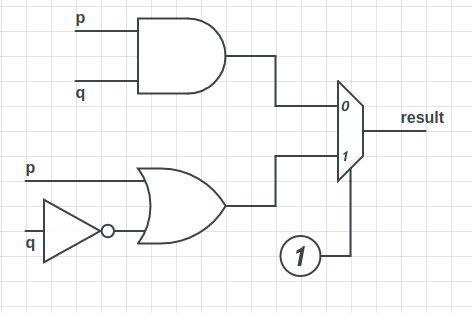
\includegraphics[scale=0.5]{circuit.png}
	\caption{Combinational Circuit}
	\label{fig: circuit}
	
\end{figure*}

In Figure \ref{fig: circuit}, the two statements are used as input. The circuit has 3 gates as AND, OR and NOT operators. It has also a 2x1 multiplexer\footnote{https://www.geeksforgeeks.org/multiplexers-in-digital-logic/} which provides to select one of the two options. 
\subproblem{a} Write the sentence that "result" output has.
\solution
\newline
Until Multiplexer it is (p $\wedge$ q ) $\wedge$ ( p $\vee$ $\neg$ q ) 
\newline
Because of selector of multiplexor is 1 that means we should consider the below one. (Input1, not input0)
\newline
( p $\vee$ $\neg$ q ) = result
\newline

\subproblem{b} Convert Figure \ref{fig: circuit} to an algorithm which you can write in any programming language that you prefer (including pseudocode).
\solution
\newline

\begin{tabbing}
if \= ( p == 1  $||$ (! q) == 1) \\
\> \= return 1;\\
\= else \\
\> \> \= return 0; 
\end{tabbing}

\end{document} 
